\label{sec:detectfalseshare}

This section first describes the basic idea of detecting false sharing. 

\subsection{Basic Idea}
\label{sec:detectionidea}
False sharing occurs when more than two threads concurrently access independent data within the same cache line, at least one of them are writes. False sharing does not necessarily cause performance problems. It can greatly degrade performance only when those accesses, caused by threads running on different cores with separate cache, actually cause a big number of cache invalidations. This is our \textbf{basic observation}. 

Generally, there are two known approaches to know how many cache invalidations actually occurring on a specific cache line, but they all suffer different shortcomings. 

The first approach relies on the underlying hardware, called as ``hardware-based approach''. We may rely on specific hardware performance counters, existing in some special hardware but not all, to know this information. But we cannot have thorough information about cache invalidations since existing mechanisms are based on sampling, which can lost a lot of information. Also, a tool based on this approach cannot apply to a different hardware that do not have specific hardware support. 

The second approach is to simulate the cache activity on different cache lines. To do that, we have to know all hardware-related information, including cache hierarchy, cache capacity and cache eviction rule, and the relationship between a thread and a specific core (that is hard to match actual situation). Even worse, simulation-based approaches are normally very slow and cannot be generalized to an execution running on a different hardware environment. 

To avoid these problems, we provide a software-only and generalized approach that can only rely on memory access history of each cache line, which is used by both \SheriffDetect{} and \Predator{} (discussed in Section~\ref{chapter:preditor}). Our approach is based on two conservative assumptions.
  
{\it First assumption:} 
All threads are running on different cores, with separate caches. Using this assumption can avoid knowing actual hardware cache hierarchy and the running situation between a thread and different cores. Although in a particular execution, two threads may run on the same core, thus reducing the effect of possible false sharing problems. Assuming that two threads are running on different cores can always represent a worst-case scenario that can happen in future executions. Thus, this assumption is very conservative, helping report any possible false sharing problem. 

{\it Second assumption:} 
A cache entry is never evicted from its private cache by cache eviction, meaning that all caches have infinite capacity. This assumption allows us to compute a cache invalidation without considering whether this entry is still in the cache or not. 

These two assumptions together allow us to compute cache invalidations based on memory accesses only. Based on these assumptions, we have the following {\bf observation}: there is a cache invalidation if a thread writes a cache line after another thread's access on the same cache line. Because the last thread accessing this cache line creates a copy of the same cache line on its running core's private cache (first assumption) and holds this copy(second assumption), this write operation definitely causes a cache invalidation, which invalidates the data copy on the core accessed by last thread. 


\begin{figure}[!t]
\centering
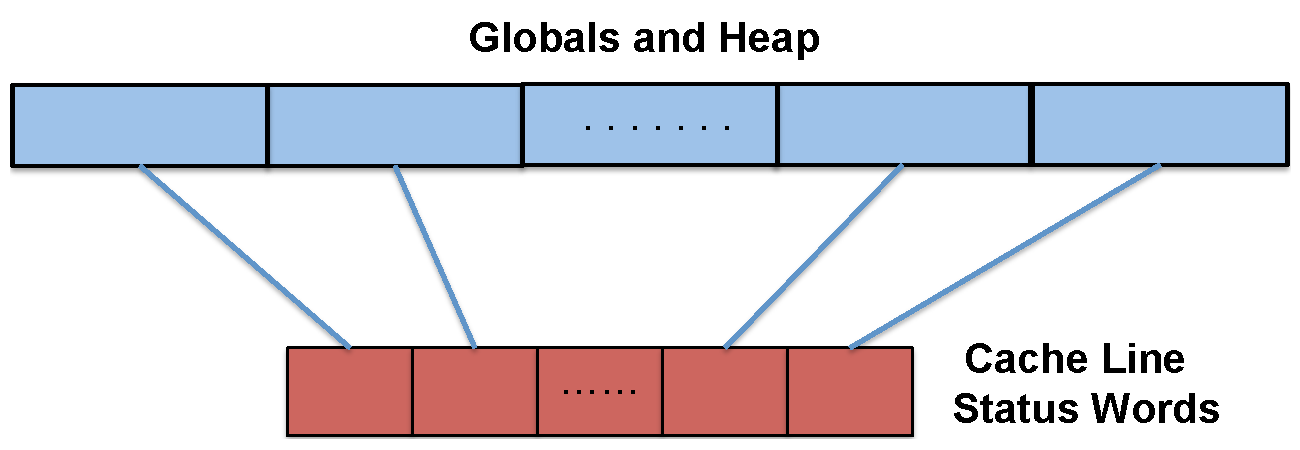
\includegraphics[width=6in]{fig/cachelinestatuswords}
\caption{
To detect false sharing, each cache line of the globals and heap maintains a cache line status word, which is updated on each memory access. \label{fig:cachelinestatusword}}
\end{figure}


To locate cache lines with a big number of cache invalidations, we maintain a cache line status word for each cache line in the globals and heap, shown in Figure~\ref{fig:cachelinestatusword}. We share a similar mechanism as another concurrent work of Zhao et.al. ~\cite{qinzhao}. 
However, the detailed implementation is totally different. Zhao et.al. utilize the detailed ownership bitmap to track those cores that have a duplicate copy of data, which can even track how many cache invalidations may happen in a write operation. However, their design cannot be easily scaled to more than 32 threads, requiring more memory overhead caused by more bits and more checking performance overhead. Also, their approach misses one important factor -- how many cache invalidations happening on a specific cache line. Without this information, it is impossible to pinpoint false sharing problems that can cause performance problems.
Our approach overcomes these shortcomings, by only tracking the last thread index and the number of cache invalidations.  Thus, we can rank the seriousness of false sharing problems based on the number of cache invalidations.
 

\subsubsection{Accurate Detection}
\label{sec:accuratedetect}
Accurate detection implies that we only report those false sharing problems that can cause performance problems. We employs the following mechanisms to avoid false positives.

First, we only report false sharing problems with a big number of cache invalidations, larger than a pre-defined but changeable threshold, thus can potentially cause performance problems. Utilizing the number of cache validations as an indicator avoids the problem of some existing tools, like PTU~\cite{detect:ptu, detect:intel}. PTU aggregates memory accesses without considering memory access interleaving, which  can report some cases that has a big number of memory accesses but without many cache invalidations. 

Second, we can differentiate false sharing from true sharing since true sharing can also cause cache invalidations. To do this, Zhao et.al. update bitmaps for every read and write in order to precisely determine whether an invalidation is related to a false sharing or a true sharing ~\cite{qinzhao}. However, this approach brings scalability problem that can not scale to more threads, bringing more memory overhead. We achieve the same target differently: we do not differentiate false sharing from true sharing during normal executions, but only track word-level accesses information: how many reads or writes are issued by which thread, where a word accessed by multiple threads is as ``shared''. This design lets us accurately distinguish false sharing from true sharing in the reporting phase, while do not have the scalability issue. It also helps diagnose where actual false sharing occurs when there are multiple fields or multiple objects in the same cache line, as this can greatly reduce the manual effort required to fix the false sharing problems.

  
Third, we can avoid pseudo false sharing (false positives) caused by memory reuses.  We intercept those memory allocations and deallocations, update information at memory deallocations for those objects without false sharing problems; heap objects involved in false sharing are never reused so that they can be reported in the end or on demand.


\subsubsection{Precise Detection}
\label{sec:precisedetect}

Precise detection implies that we can precisely point out where the problem is. Thus, programmers can leverage on that to identify and correct false sharing problems.

For global variables, we identify the name of global variables involving in false sharing problems, by looking up corresponding debug information. For heap objects, we report the callsite of those memory allocations by presenting the line of source code. In order to capture the origins of heap objects, we intercept those intercepting memory allocations and deallocations and use different ways to get callsite information, which are discussed in Section~\ref{sec:sheriffcallsite} and Section~\ref{sec:predatorcallsite}.

To help programmers precisely identify culprits of performance problem, we also present word-level accesses information so that the exact variables or fields that cause performance problems can be determined precisely. 

\subsubsection{Flexible Reporting}
\label{sec:flexiblereport}

We provide two different ways to report those false sharing problems. Normally, we can report those false sharing problems in the end of a program. However, this way does not work for those long-running applications. Thus, we provide a on-demand reporting way. User can send a specified signal to those applications that are installed with our tool. By intercepting those signals, we can report false sharing problems on demand.

In order to find out those cache lines with false sharing problems, we scan cache line status words of all memory, including the globals and heap, and only report those false sharing problems that can possibly cause performance problems, with the number of cache invalidations larger than a pre-defined but adjustable threshold.

\subsection{Detailed Implementations}

\label{sec:sheriffdetect}
\SheriffDetect{} relies on the \sheriff{} framework to track memory writes, thus detecting the write-write type of false sharing problems.  

%%% Tongping Liu
\subsubsection{Tracking Memory Accesses}
\label{sec:memoryaccesses}

\begin{figure*}[!t]
\centering
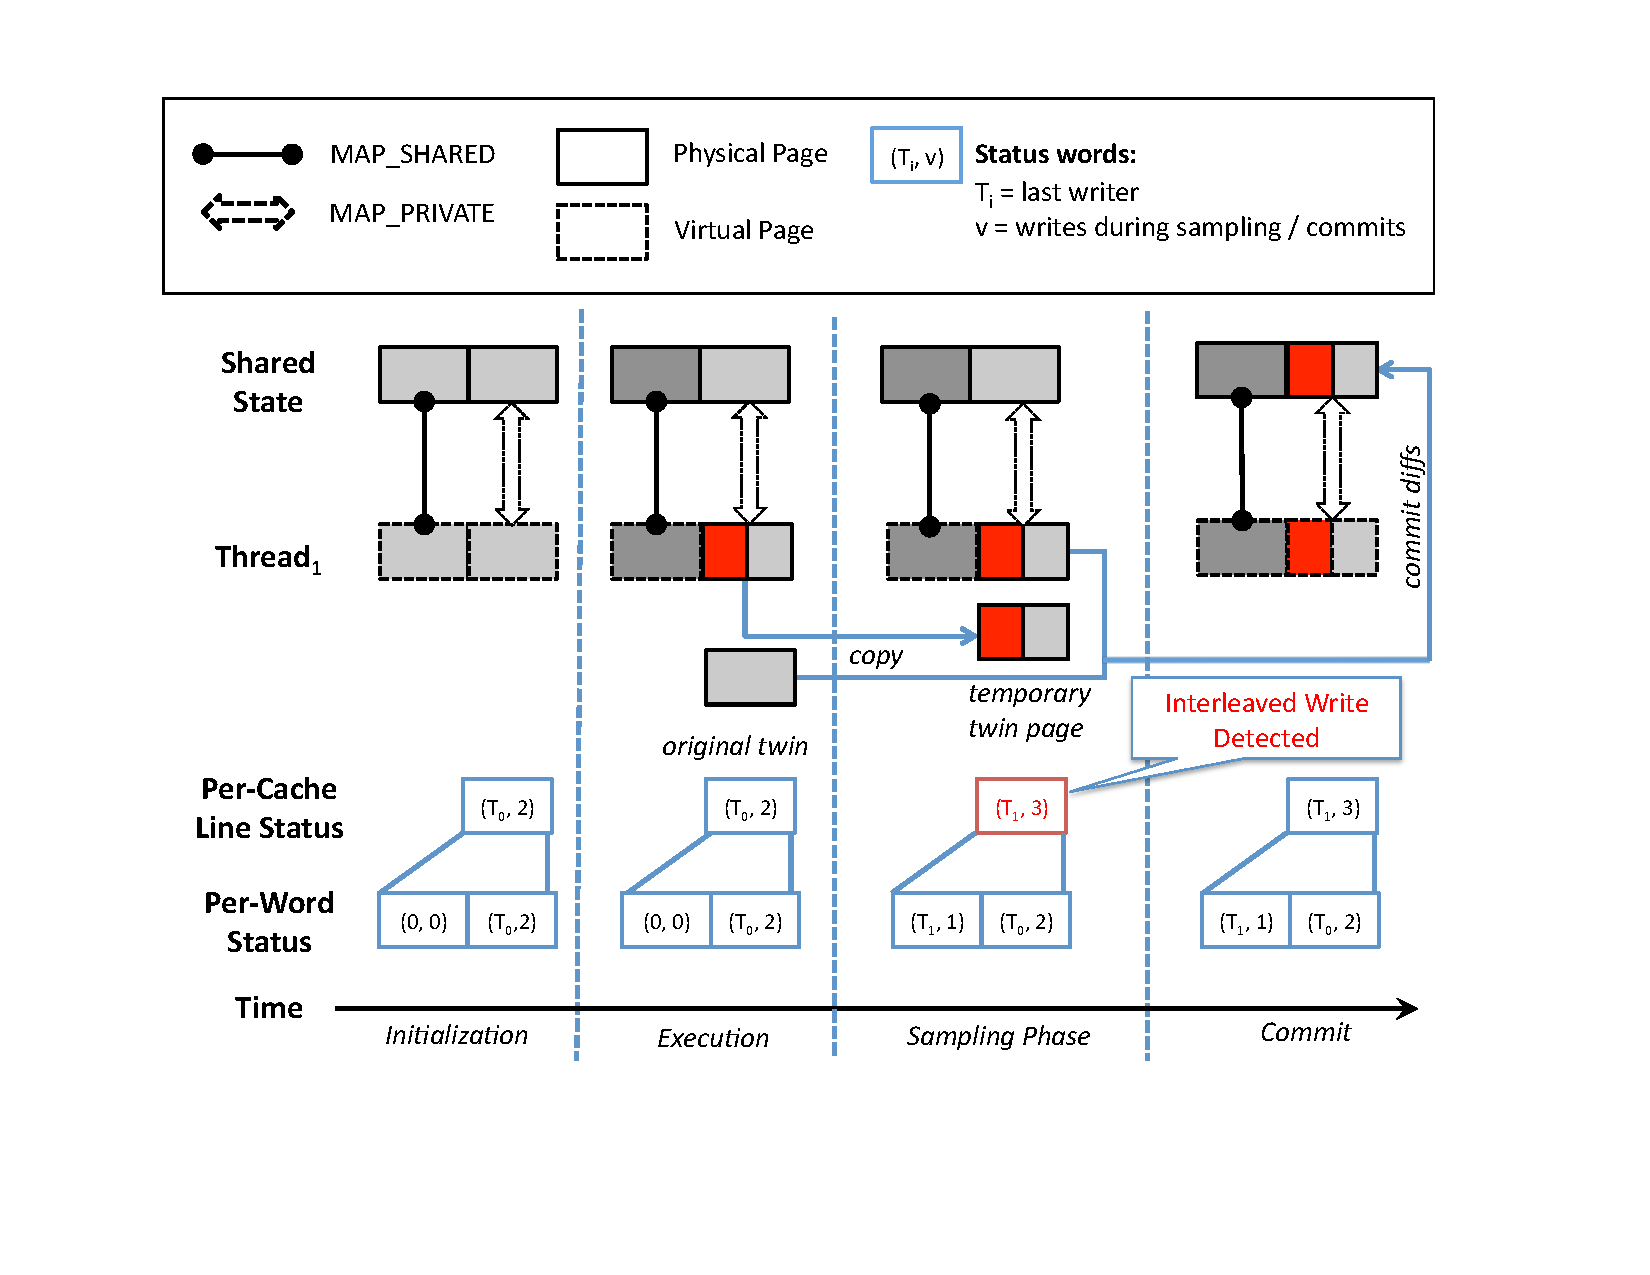
\includegraphics[width=6in]{sheriff/figure/sheriffdetective.pdf}
\caption{
Overview of \SheriffDetect{}’s operations. \SheriffDetect{} extends \Sheriff{} with sampling, per-cacheline status arrays, and per-word status arrays. For clarity of exposition, the diagram depicts just one cache line per page and two words per cache line.\label{fig:sheriffdetect}}
\end{figure*}

As discussed in Section~\ref{sec:detectionidea}, we can detect cache invalidations only based on memory accesses: for every memory access, we check recent memory access history, update the number of cache invalidations if possible, and update corresponding memory access history. 
Base on our observation, if the current access is a write, and other threads have accessed this cache line since last invalidation, then there is a cache invalidation. 
The \sheriff{} framework isolates executions from different threads, only commits those changes of different threads to the shared mapping at synchronization boundaries. Thus, by comparing a ``working'' page against its ``twin'' page,  \sheriffDetect{} can discover those accumulative memory writes  that occurred in the last transaction.  

However, if a transaction is long-running, finding memory changes at the end of every transaction is not enough 
to find those false sharing problems happening in the middle of a transaction. For example, the \texttt{linear\_regression} benchmark (described in Section~\ref{sec:evaluation}), 
degrading the performance by more than $10\times$ because of its false sharing problem, only has a single transaction per thread. 

In order to detect memory writes in the middle of an transaction, \SheriffDetect{} employs a sampling mechanism, employing the timer mechanism of the underlying operating system. 
We utilize the \texttt{alarm} library API to generate a periodical alarm to our detection system: by handlingthe \texttt{SIGALRM} signal, \SheriffDetect{} tracks memory writes accumulatively in the current period using the twinning and diffing mechanism (section~\ref{sec:twinning-and-diffing}). To do this, \SheriffDetect{} also keeps and updates a ``temporary twin'' page at every alarm interval, by simply copying from its ``working'' page. The difference between a ``working'' page and its ``temporary'' page implies those memory writes happening in the current sampling period. 

Currently, \SheriffDetect{} samples memory accesses of each thread at every 10 microsecond, which is  adjustable in our implementation. More frequent sampling may uncover more false sharing problems, but at the cost of increasing performance overhead. The tradeoff between effectiveness and performance overhead is further discussed and evaluated in Section~\ref{sec:results-sampling-overhead}. 

\subsubsection{Tracking Cache Invalidations}
\label{sec:invalidation}
As the discussion in Section~\ref{sec:detectionidea}, \SheriffDetect{} tracks and reports those cache lines with a big number of cache invalidations, which may cause serious performance problems. 

In order to track cache invalidations, \SheriffDetect{} introduces a cache line status word for every cache line of the globals and heap, showed in Figure~\ref{fig:cachelinestatusword}.  \SheriffDetect{} introduces two fields for every cache line status word, the last thread writing to this cache line and the number of cache invalidations of this cache line. 
Every time, when \SheriffDetect{} tracks a memory write, either at the end of each transaction or during the sampling timer handler, it updates these two fields correspondingly. Based on the assumptions described in Section~\ref{sec:detectionidea}, \SheriffDetect{} increments the number of cache invalidations when there is a write from a different thread and changes the last thread to the current thread (by recording thread id). To avoid using lock, \SheriffDetect{} updates those counters using atomic primitives. Since we base on thread id to identify whether there is a cache invalidation, without keeping track of detailed ownership id, this approach can scale up to any number of threads.   

\subsection{Optimizations}

\SheriffDetect{} employs the following optimizations in order to reduce its performance overhead. 

\paragraph{Getting Callsite Information.}
\label{sec:sheriffcallsite}

\SheriffDetect{} intercepts memory allocation operations in order to collect callsites for every heap object. To reduce the performance overhead, \SheriffDetect{} does not use the \texttt{bracktrace()} function call, but identify the callsite by analyzing the return or frame address using GCC extensions. However, this can not work on applications without debugging information. 

\paragraph{Reducing timer overhead.}
As explained in Section~\ref{sec:memoryaccesses}, \SheriffDetect{} uses a sampling mechanism to track cache invalidations. To reduce the performance overhead caused by by handling those alarm signals, \SheriffDetect{} activates sampling only when the average transaction time is larger than a pre-defined threshold (currently 10 milliseconds). \SheriffDetect{} uses an exponential moving average to track the average transaction time ($\alpha = 0.9$). This optimization does not significantly reduce the possibility of finding false sharing, since \SheriffDetect{} can track those accumulative writes inside every short transaction by checking only at the end of transactions.

\paragraph{Sampling to find shared pages.} 
If an application has a large number of transactions or a large memory footprint, the overhead of handling page protection can dominate the total running time.
To reduce the number of pages that should be tracked, \SheriffDetect{} leverages a
simple insight: if two threads can falsely share (write-write share) a cache line, then they must simultaneously write to the same page containing this cache line. 
Leveraging on this insight, \SheriffDetect{} only tracks those pages written by multiple threads. 

In order to identify those shared pages, \SheriffDetect{} is based on the following assumption: if objects on a page are frequently falsely shared, the corresponding page must also be frequently shared; thus, even relatively infrequent sampling on memory accesses can reveal the shared relationship. \SheriffDetect{} currently samples the first 50 out of every 1,000 periods (one period equals one transaction or one sampling interval). At the beginning of each sampling period, all memory pages are made read-only so that any
writes to each page will be detected. Upon finding a page that is shared across multiple threads, \SheriffDetect{} tracks all memory accesses happening on this page, thus possibly finding any false sharing inside this page. 

By using this sampling mechanism, those pages, with sharing status unknown, impose no protection overhead at all. \sheriffDetect{} only pays protection overhead for those shared pages outside the sampling period, instead of all memory pages. 

\subsection{Limitation}
\label{discussion:faultofdetect}

Unlike previous tools, \SheriffDetect{} reports no false positives, differentiates true sharing from false sharing, and avoids false positives caused by the reuse of heap objects. 

However, \SheriffDetect{} can under-report false sharing instances in the following situations:

\paragraph{Single writer.}
False sharing usually involves concurrent updates from multiple threads. But it can also arise when there is exactly one thread writing to part of a cache line while other threads read from this cache line. 
Because \sheriffdetect{} can only track writes, it cannot detect this single-writer false sharing, missing some false sharing problems. 

\paragraph{Heap-induced false sharing.}  
\sheriff{} replaces the standard memory allocator with one that, like the Hoard allocator, avoids most heap-induced false sharing. \sheriff{}'s memory allocator (like Hoard), carves memory into page-sized chunks; each thread allocates from its own set of chunks, and the allocator never splits cache lines across threads. Because \SheriffDetect{} uses a different custom memory allocator, it cannot detect false sharing that is caused by using the standard memory allocator. Since it is straightforward to deploy Hoard or a similar allocator to avoid heap-induced false sharing, this limitation is not a problem in practice.

\paragraph{Misses due to sampling.}  Since it uses sampling to find shared pages, \SheriffDetect{} may fail to track those pages that written in the middle of sampling intervals. We hypothesize that false sharing instances that affect performance are unlikely to perform frequent writes exclusively during that time, and so are unlikely to be missed.
